\subsubsection{Middleware}
\subsubsubsection{Application - Middleware}
The communication protocol between application layer and middleware layer 
\paragraph{Fire and forget} 
It is a one-way message pattern (the service sends a message without expecting 
a response). Since the application and the middleware will reside on the same 
physical node we can assume that the communication is reliable, once a message 
is sent from the application layer it arrives to the middleware layer and 
viceversa. The asynchronous communication decouples (when possible) 
the computation of the application from the computation of the middleware 
and viceversa. The standard interfaces for communication 
implemented by application layer and middleware layer enables the use of 
heterogeneous technologies for each one. Defining a standard interface 
is fundamental to abstract from the underlying technologies (implementation).

\subsubsubsection{Middleware - Middleware}

\subsubsubsection{System Boostrap}
As pointed out in the problem analysis, the system has to start neatly. Hence,
we need to design a protocol to respect in order to accomplish this goal.

The protocol is represented in figure \ref{fig:sys-bootstrap-protocol}, where:

\begin{itemize}
  \item a circle is a logical node that is composed of a middleware layer
    \textbf{MW} and an application layer \textbf{APP}. Since the middleware
    has to be application-independent, it only assumes that there is an
    interface through which it is possible to make an application start neatly;
  \item a named arrow represents a message that is sent from a logical node
    through another one with the name as its payload;
  \item the numbers in the figure represents the progress of the system
    bootstrap.
\end{itemize}

\begin{figure}[H]
  \centering
  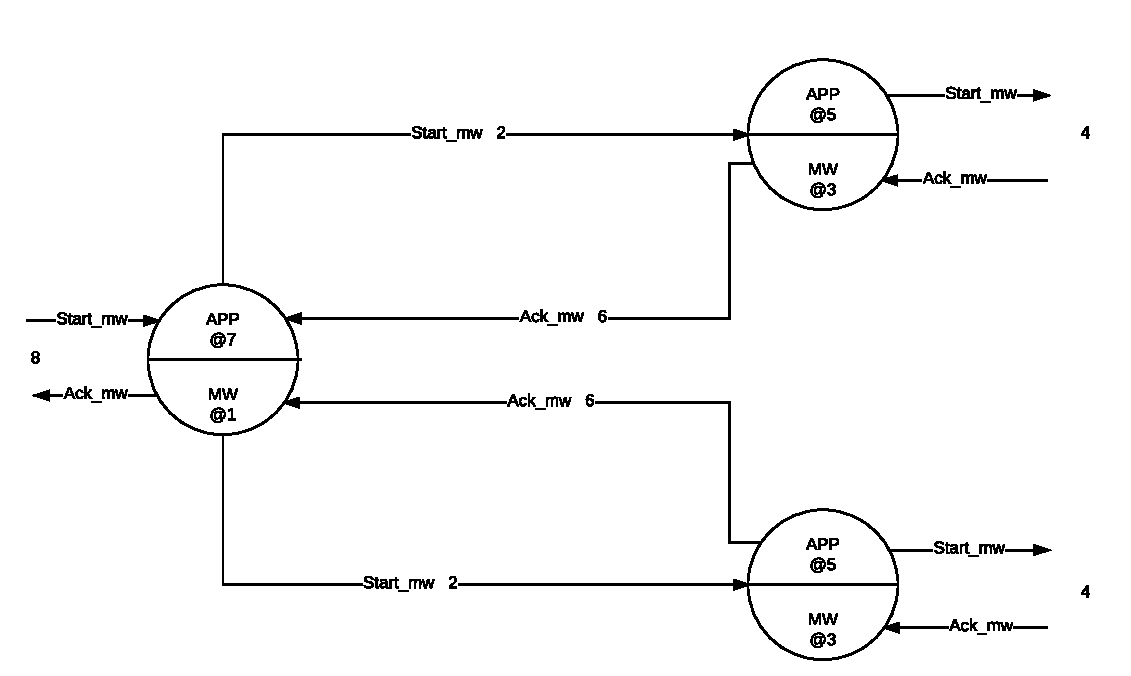
\includegraphics[width=\columnwidth]{sections/images/solution/bootstrap.pdf}
  \caption{System bootstrap protocol}
  \label{fig:sys-bootstrap-protocol}
\end{figure}

Assuming that a \texttt{Start\_mw} message arrives to a non-booted node (say
$l$) at time instant 0, the protocol is defined as follows:

\begin{enumerate}
  \item The leftmost node $l$ in figure \ref{fig:sys-termination-protocol}
    starts its own middleware services;
  \item $l$ sends a \texttt{Start\_mw} message to the set $S$ of all the nodes
    it knows;
  \item $l$ waits for each node in $S$ to boot, i.e. $l$ waits for all nodes
    in $S$ to send an \texttt{Ack\_mw} message back;
  \item The middleware MW of $l$ asks to start the application APP;
  \item $l$ then sends an \texttt{Ack\_mw} message back.
\end{enumerate}

As it can be seen in the figure, this behaviour is replicated recursively
by all nodes of the system. If a node has already been booted, then it only
sends \texttt{Ack\_mw} back.

\subsubsubsection{System Termination}
Also, the system has to shutdown neatly. Therefore we designed a protocol to
stop the entire system; please notice that this one could be seen as a
symmetric version of the System Bootstrap protocol.
% TODO: please check the sentence here above

The protocol is represented in figure \ref{fig:sys-termination-protocol}, where
the conventions are the same as the ones used in figure
\ref{fig:sys-bootstrap-protocol}.

\begin{figure}[H]
  \centering
  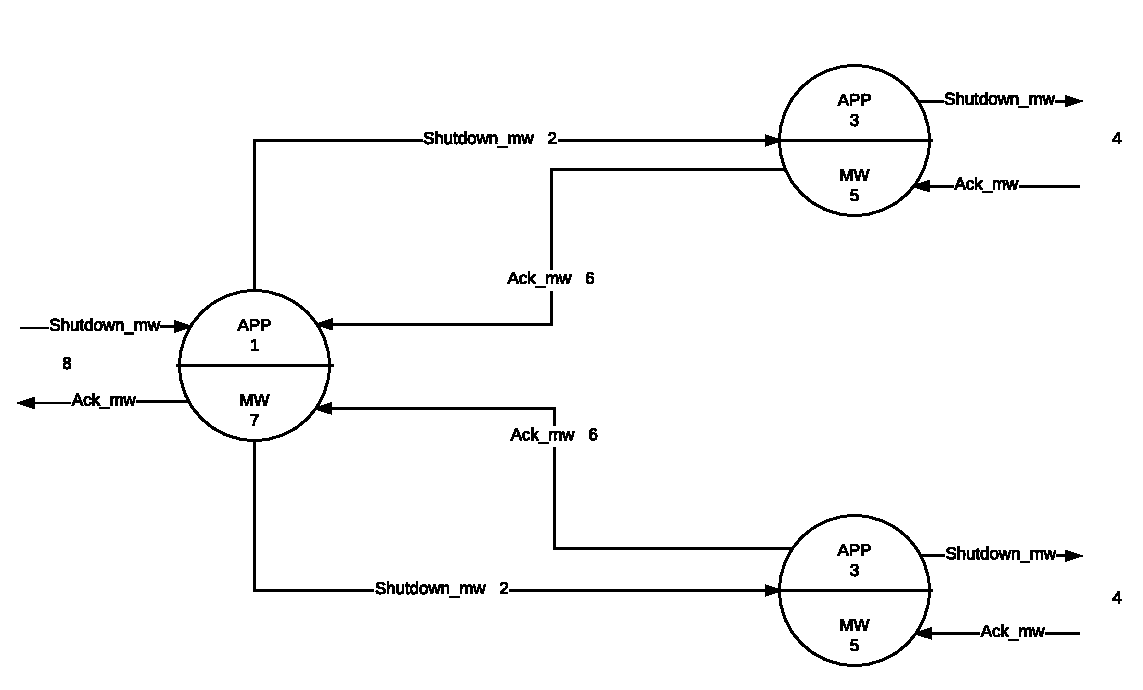
\includegraphics[width=\columnwidth]{sections/images/solution/termination.pdf}
  \caption{System termination protocol}
  \label{fig:sys-termination-protocol}
\end{figure}

Assuming that a \texttt{Shutdown\_mw} message arrives to a non-terminated node
$l$ (let it be the leftmost one in the picture) at time instant 0, the protocol
is defined as follows:

\begin{enumerate}
  \item The middleware MW of $l$ asks to terminate the application APP;
  \item $l$ sends a \texttt{Shutdown\_mw} message to the set
    $S$ of all the nodes it knows;
  \item $l$ waits for each node in $S$ to terminate, i.e. $l$ waits for all
    nodes in $S$ to send an \texttt{Ackt\_mw} message back;
  \item $l$ stops its own middleware services;
  \item $l$ then sends an \texttt{Ackt\_mw} message back.
\end{enumerate}

As it can be seen in the related figure, this behaviour is replicated
recursively by all nodes of the system. If a node has already terminated, then
it only sends \texttt{Ackt\_mw} back.
